\documentclass[]{article}
\usepackage[margin=0.5cm]{geometry}
\usepackage{algorithm}
\usepackage{algpseudocode}
\usepackage{mathtools}
\usepackage{tikz}
\usepackage{xcolor}

\begin{document}

\algrenewcommand\algorithmicrequire{\textbf{Input:}}
\algrenewcommand\algorithmicensure{\textbf{Output:}}

\newcommand{\handle}[1]{\textbf{handle}(#1)}
\newcommand{\key}[1]{\textbf{key}(#1)}
\newcommand{\valueof}[1]{\textbf{value}(#1)}
\newcommand{\wrap}[1]{\textbf{wrap}(#1)}
\newcommand{\unwrap}[1]{\textbf{uwrap}(#1)}
\newcommand{\encrypt}[1]{\textbf{encrypt}(#1)}
\newcommand{\decrypt}[1]{\textbf{decrypt}(#1)}
\newcommand{\node}[1]{#1}
\newcommand{\edge}[2]{(#1,#2)}
\newcommand{\graph}[1]{#1}
\newcommand{\encryption}[2]{{\{#1\}}_{#2}}
\newcommand{\known}[1]{\textbf{known}(#1)}
\newcommand{\copygraph}[1]{\textbf{copy}(#1)}

A node can either be a key node or a handle node.

\begin{enumerate}
    \item All keys have distinct values. In other words, there cannot be two distinct keys with the same value.
    \item All keys have at most two handles. In other words, there cannot be a key with more than two handles.
\end{enumerate}

Directed graphs with multiedges are denoted with $G_0$, $G_1$; nodes with $n_1, n_2$.

\begin{figure}[h!]
    \centering
    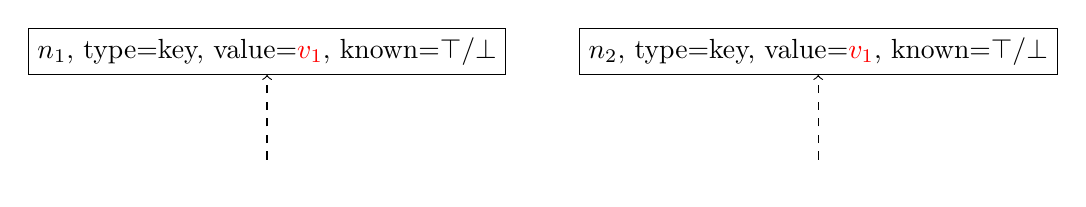
\begin{tikzpicture}
        \node (n1) at ( 0.0, 1.5) [draw, rectangle] {$n_1$, type=key, value=\textcolor{red}{$v_1$}, known=$\top/\bot$};
        \node (n2) at ( 7.0, 1.5) [draw, rectangle] {$n_2$, type=key, value=\textcolor{red}{$v_1$}, known=$\top/\bot$};
        \node (n3) at ( 0.0, 0.0) {};
        \node (n4) at ( 7.0, 0.0) {};

        \draw[->, dashed] (n3) -- (n1) node[midway, sloped, above] {};
        \draw[->, dashed] (n4) -- (n2) node[midway, sloped, above] {};
    \end{tikzpicture}
    \caption{Violates condition 1.}
\end{figure}

\begin{figure}[h!]
    \centering
    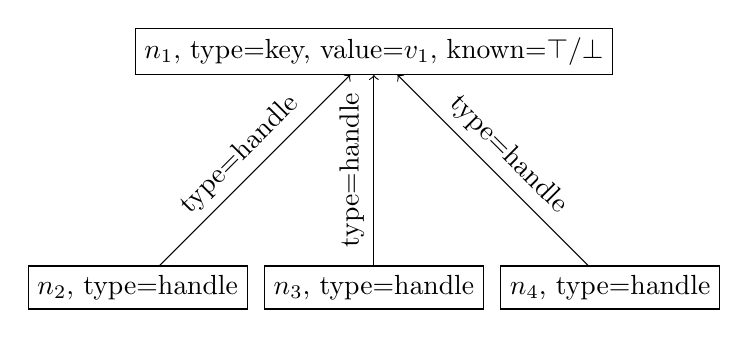
\begin{tikzpicture}
        \node (n1) at (  0.0, 3.0) [draw, rectangle] {$n_1$, type=key, value=$v_1$, known=$\top/\bot$};
        \node (n2) at ( -3.0, 0.0) [draw, rectangle] {$n_2$, type=handle};
        \node (n3) at (  0.0, 0.0) [draw, rectangle] {$n_3$, type=handle};
        \node (n4) at (  3.0, 0.0) [draw, rectangle] {$n_4$, type=handle};

        \draw[->] (n2) -- (n1) node[midway, sloped, above] {type=handle};
        \draw[->] (n3) -- (n1) node[midway, sloped, above] {type=handle};
        \draw[->] (n4) -- (n1) node[midway, sloped, above] {type=handle};
    \end{tikzpicture}
    \caption{Violates condition 2.}
\end{figure}

We use AALpy to understand the behavior of a PKCS \#11 implementation.
We need to provide to AALpy a reasonable alphabet of commands.

We start from an initial state (that is, handles and keys, known or not by the attacker). We need to generate a reasonsable alphabet for AALpy.
``Reasonable'' means that it should not contain commands which are useless, that is, commands that produce useless knowledge.

\begin{figure}[h!]
    \centering
    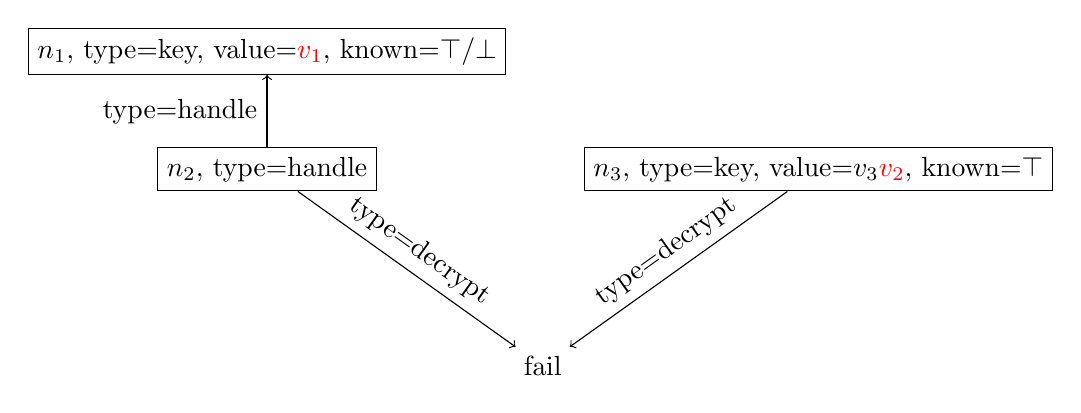
\begin{tikzpicture}
        \node (n1) at ( 0.0,  0.0) [draw, rectangle] {$n_1$, type=key, value=$\textcolor{red}{v_1}$, known=$\top/\bot$};
        \node (n2) at ( 0.0, -1.5) [draw, rectangle] {$n_2$, type=handle};
        \node (n3) at ( 7.0, -1.5) [draw, rectangle] {$n_3$, type=key, value=$\encryption{v_3}{\textcolor{red}{v_2}}$, known=$\top$};
        \node (n4) at ( 3.5, -4.0) [] {fail};

        \draw[->] (n2) -- (n1) node[midway, left] {type=handle};
        \draw[->] (n2) -- (n4) node[midway, sloped, above] {type=decrypt};
        \draw[->] (n3) -- (n4) node[midway, sloped, above] {type=decrypt};
    \end{tikzpicture}
    \caption{The command \texttt{decrypt(n2, n3)} is useless.}
\end{figure}

\begin{figure}[h!]
    \centering
    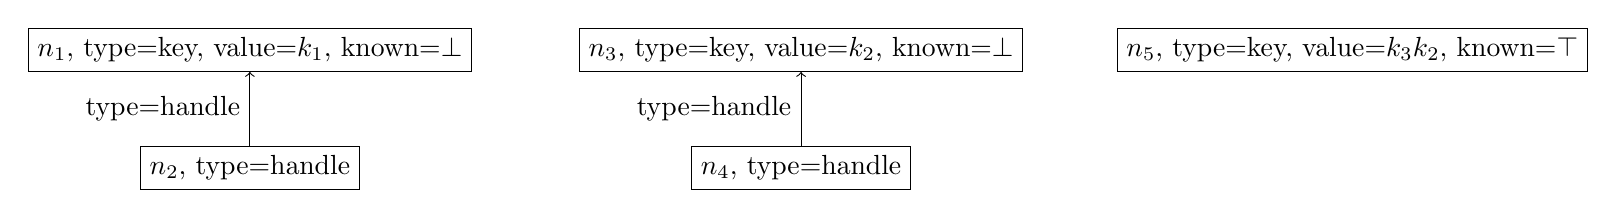
\begin{tikzpicture}
        \node (n1) at ( 0.0,  1.5) [draw, rectangle] {$n_1$, type=key, value=$k_1$, known=$\bot$};
        \node (n2) at ( 0.0,  0.0) [draw, rectangle] {$n_2$, type=handle};
        \node (n3) at ( 7.0,  1.5) [draw, rectangle] {$n_3$, type=key, value=$k_2$, known=$\bot$};
        \node (n4) at ( 7.0,  0.0) [draw, rectangle] {$n_4$, type=handle};
        \node (n5) at ( 14.0, 1.5) [draw, rectangle] {$n_5$, type=key, value=$\encryption{k_3}{k_2}$, known=$\top$};

        \draw[->] (n2) -- (n1) node[midway, left] {type=handle};
        \draw[->] (n4) -- (n3) node[midway, left] {type=handle};
    \end{tikzpicture}
    \caption{Initial state of the Re-import attack 2.}
\end{figure}

\newpage

\section*{Wrap}

\begin{figure}[h!]
    \centering
    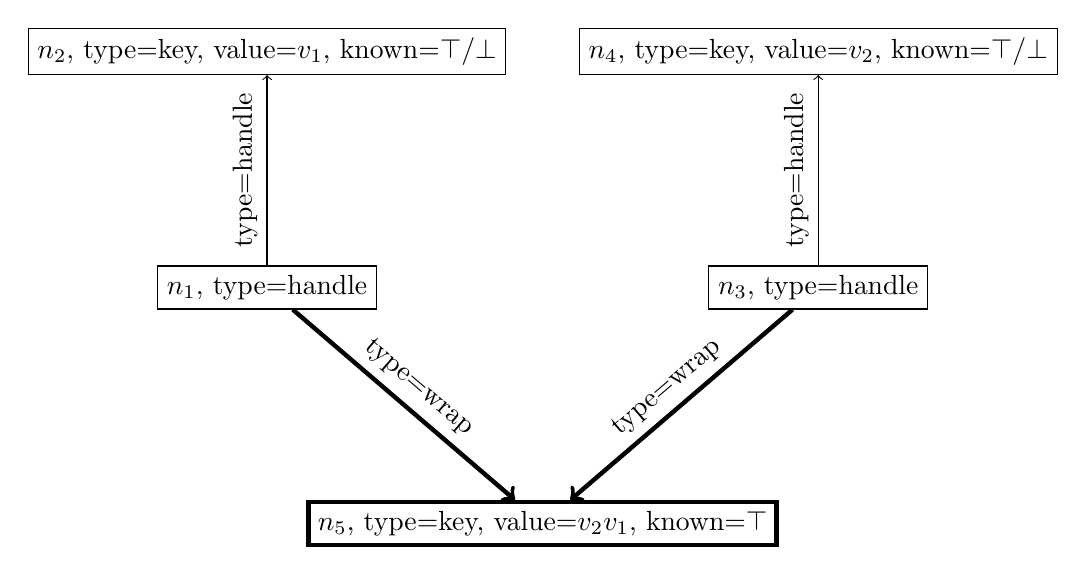
\begin{tikzpicture}
        \node (n2) at ( 0.0,  3.0) [draw, rectangle] {$n_2$, type=key, value=$v_1$, known=$\top/\bot$};
        \node (n4) at ( 7.0,  3.0) [draw, rectangle] {$n_4$, type=key, value=$v_2$, known=$\top/\bot$};
        \node (n1) at ( 0.0,  0.0) [draw, rectangle] {$n_1$, type=handle};
        \node (n3) at ( 7.0,  0.0) [draw, rectangle] {$n_3$, type=handle};
        \node (n5) at ( 3.5, -3.0) [draw, rectangle, ultra thick] {$n_5$, type=key, value=$\encryption{v_2}{v_1}$, known=$\top$};

        \draw[->] (n1) -- (n2) node[midway, sloped, above] {type=handle};
        \draw[->] (n3) -- (n4) node[midway, sloped, above] {type=handle};
        \draw[->, ultra thick] (n1) -- (n5) node[midway, sloped, above] {type=wrap};
        \draw[->, ultra thick] (n3) -- (n5) node[midway, sloped, above] {type=wrap};
    \end{tikzpicture}
    \caption{Node $n_5$ does not exist. We add $n_5$ and edges $(n_1, n_5), (n_3, n_5)$ to it. We add command \texttt{wrap(n1, n3)} to the alphabet.}
\end{figure}

\begin{figure}[h!]
    \centering
    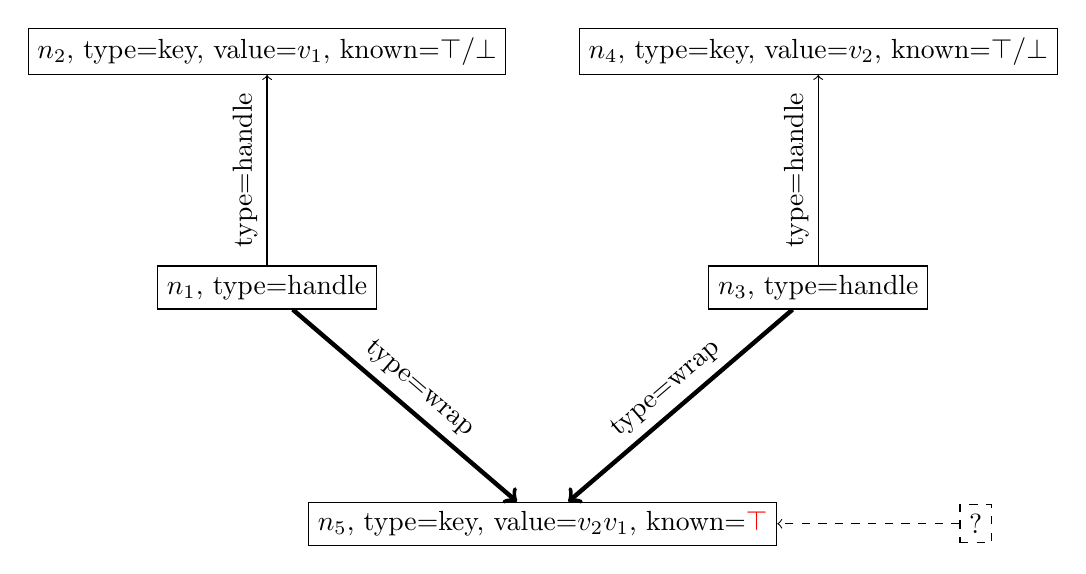
\begin{tikzpicture}
        \node (n2) at ( 0.0,  3.0) [draw, rectangle] {$n_2$, type=key, value=$v_1$, known=$\top/\bot$};
        \node (n4) at ( 7.0,  3.0) [draw, rectangle] {$n_4$, type=key, value=$v_2$, known=$\top/\bot$};
        \node (n1) at ( 0.0,  0.0) [draw, rectangle] {$n_1$, type=handle};
        \node (n3) at ( 7.0,  0.0) [draw, rectangle] {$n_3$, type=handle};
        \node (n5) at ( 3.5, -3.0) [draw, rectangle] {$n_5$, type=key, value=$\encryption{v_2}{v_1}$, known=\textcolor{red}{$\top$}};
        \node (p3) at ( 9.0, -3.0) [draw, rectangle, dashed] {?};

        \draw[->] (n1) -- (n2) node[midway, sloped, above] {type=handle};
        \draw[->] (n3) -- (n4) node[midway, sloped, above] {type=handle};
        \draw[->, ultra thick] (n1) -- (n5) node[midway, sloped, above] {type=wrap};
        \draw[->, ultra thick] (n3) -- (n5) node[midway, sloped, above] {type=wrap};
        \draw[->, dashed] (p3) -- (n5);
    \end{tikzpicture}
    \caption{Node $n_5$ already exists. If the pair of edges $(n_1, n_5), (n_3, n_5)$ does not already exist, we add it. We set $n_5$ as known. We add command \texttt{wrap(n1, n3)} to the alphabet.}
\end{figure}

\newpage

\section*{Encrypt}

\begin{figure}[h!]
    \centering
    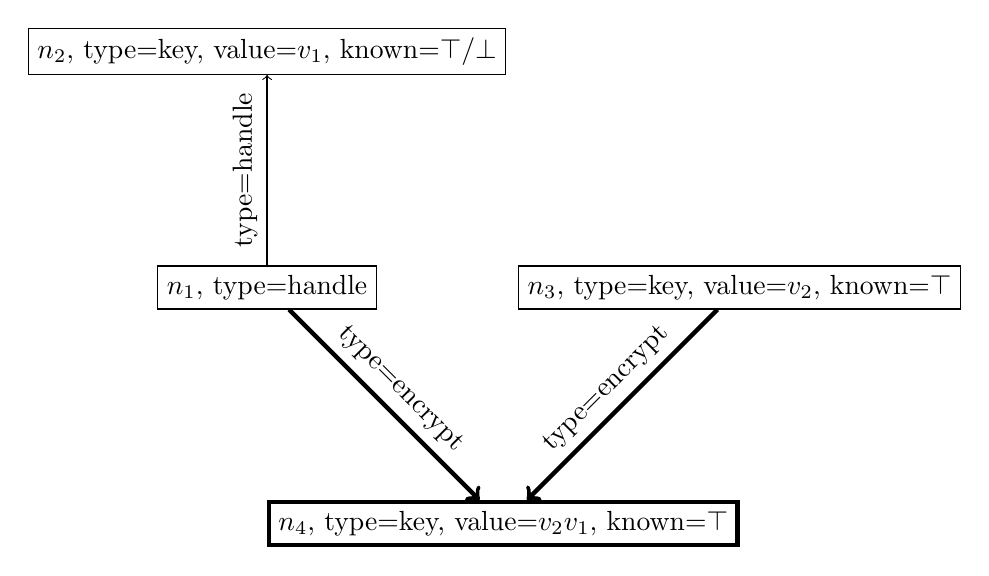
\begin{tikzpicture}
        \node (n2) at ( 0.0,  3.0) [draw, rectangle] {$n_2$, type=key, value=$v_1$, known=$\top/\bot$};
        \node (n3) at ( 6.0,  0.0) [draw, rectangle] {$n_3$, type=key, value=$v_2$, known=$\top$};
        \node (n1) at ( 0.0,  0.0) [draw, rectangle] {$n_1$, type=handle};
        \node (n4) at ( 3.0, -3.0) [draw, rectangle, ultra thick] {$n_4$, type=key, value=$\encryption{v_2}{v_1}$, known=$\top$};

        \draw[->] (n1) -- (n2) node[midway, sloped, above] {type=handle};
        \draw[->, ultra thick] (n1) -- (n4) node[midway, sloped, above] {type=encrypt};
        \draw[->, ultra thick] (n3) -- (n4) node[midway, sloped, above] {type=encrypt};
    \end{tikzpicture}
    \caption{Node $n_4$ does not exist. We add $n_4$ and edges $(n_1, n_4), (n_3, n_4)$ to it. We add command \texttt{encrypt(n1, n3)} to the alphabet.}
\end{figure}


\begin{figure}[h!]
    \centering
    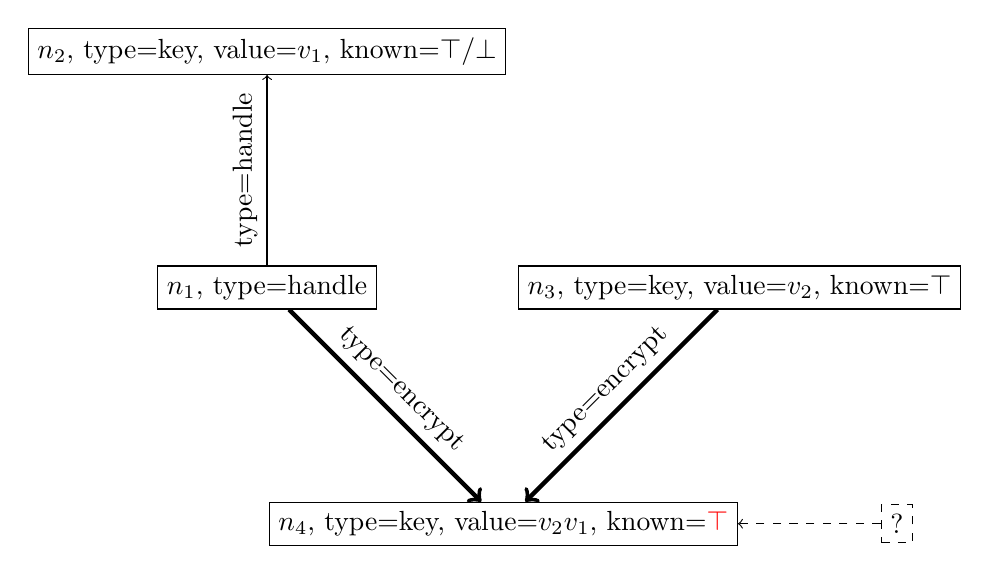
\begin{tikzpicture}
        \node (n2) at ( 0.0,   3.0) [draw, rectangle] {$n_2$, type=key, value=$v_1$, known=$\top/\bot$};
        \node (n3) at ( 6.0,   0.0) [draw, rectangle] {$n_3$, type=key, value=$v_2$, known=$\top$};
        \node (n1) at ( 0.0,   0.0) [draw, rectangle] {$n_1$, type=handle};
        \node (n4) at ( 3.0,  -3.0) [draw, rectangle] {$n_4$, type=key, value=$\encryption{v_2}
                {v_1}$, known=\textcolor{red}{$\top$}};
        \node (p3) at ( 8.0,  -3.0) [draw, rectangle, dashed] {?};

        \draw[->] (n1) -- (n2) node[midway, sloped, above] {type=handle};
        \draw[->, ultra thick] (n1) -- (n4) node[midway, sloped, above] {type=encrypt};
        \draw[->, ultra thick] (n3) -- (n4) node[midway, sloped, above] {type=encrypt};
        \draw[->, dashed] (p3) -- (n4);
    \end{tikzpicture}
    \caption{Node $n_4$ already exists. If the pair of edges $(n_1, n_4), (n_3, n_4)$ does not already exist, we add it. We set $n_4$ as known. We add command \texttt{encrypt(n1, n3)} to the alphabet.}
\end{figure}

\newpage

\section*{Unwrap}

\begin{figure}[h!]
    \centering
    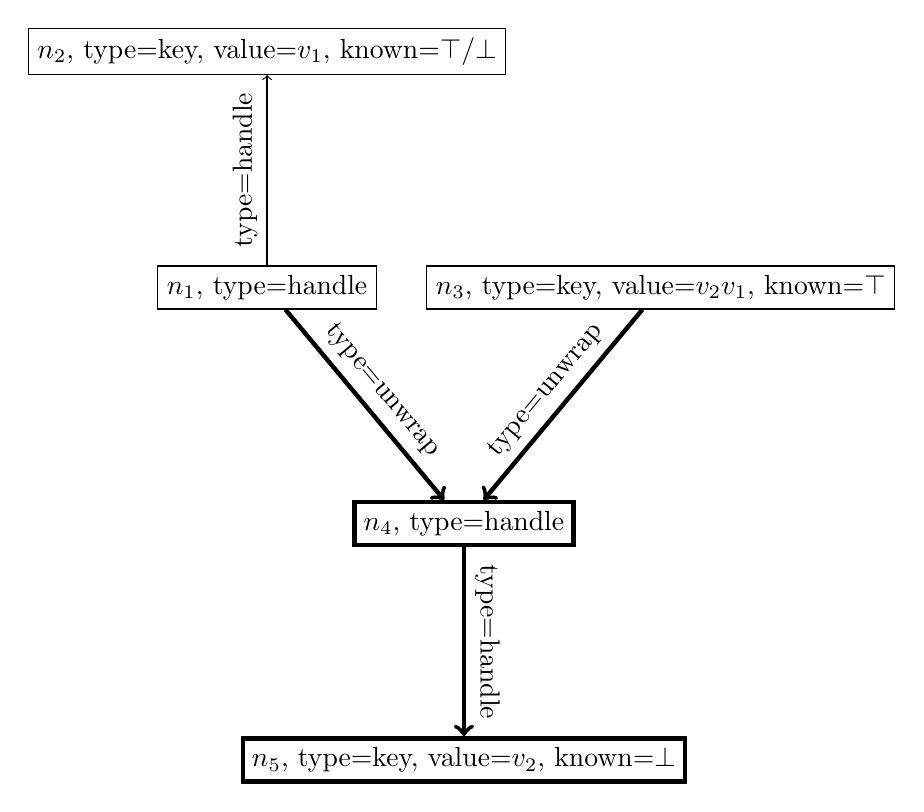
\begin{tikzpicture}
        \node (n2) at ( 0.0,   3.0) [draw, rectangle] {$n_2$, type=key, value=$v_1$, known=$\top/\bot$};
        \node (n3) at ( 5.0,   0.0) [draw, rectangle] {$n_3$, type=key, value=$\encryption{v_2}{v_1}$, known=$\top$};
        \node (n1) at ( 0.0,   0.0) [draw, rectangle] {$n_1$, type=handle};
        \node (n4) at ( 2.5,  -3.0) [draw, rectangle, ultra thick] {$n_4$, type=handle};
        \node (n5) at ( 2.5,  -6.0) [draw, rectangle, ultra thick] {$n_5$, type=key, value=$v_2$, known=$\bot$};

        \draw[->] (n1) -- (n2) node[midway, sloped, above] {type=handle};
        \draw[->, ultra thick] (n1) -- (n4) node[midway, sloped, above] {type=unwrap};
        \draw[->, ultra thick] (n3) -- (n4) node[midway, sloped, above] {type=unwrap};
        \draw[->, ultra thick] (n4) -- (n5) node[midway, sloped, above] {type=handle};
    \end{tikzpicture}
    \caption{Node $n_5$ does not exist. We add $n_5$ and $n_4$. We add edge $(n_4, n_5)$ and edges $(n_1, n_4), (n_3, n_4)$. We add command \texttt{unwrap(n1, n3)} to the alphabet.}
\end{figure}

\begin{figure}[h!]
    \centering
    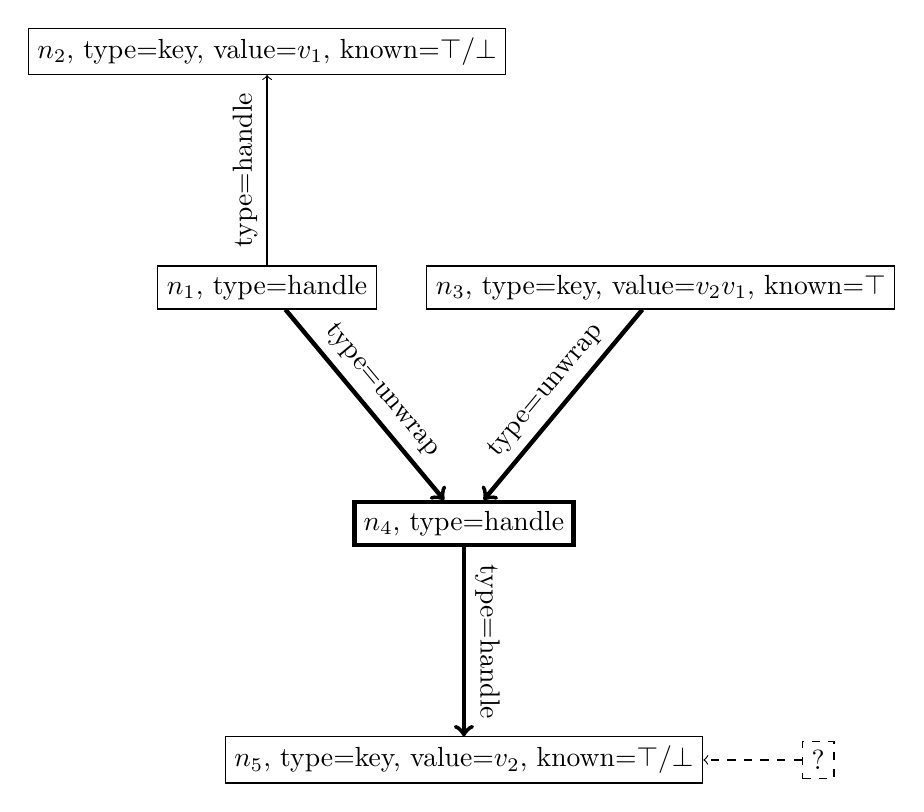
\begin{tikzpicture}
        \node (n2) at ( 0.0,   3.0) [draw, rectangle] {$n_2$, type=key, value=$v_1$, known=$\top/\bot$};
        \node (n3) at ( 5.0,   0.0) [draw, rectangle] {$n_3$, type=key, value=$\encryption{v_2}{v_1}$, known=$\top$};
        \node (n1) at ( 0.0,   0.0) [draw, rectangle] {$n_1$, type=handle};
        \node (n4) at ( 2.5,  -3.0) [draw, rectangle, ultra thick] {$n_4$, type=handle};
        \node (n5) at ( 2.5,  -6.0) [draw, rectangle] {$n_5$, type=key, value=$v_2$, known=$\top/\bot$};
        \node (p4) at ( 7.0,  -6.0) [draw, rectangle, dashed] {?};

        \draw[->] (n1) -- (n2) node[midway, sloped, above] {type=handle};
        \draw[->, ultra thick] (n1) -- (n4) node[midway, sloped, above] {type=unwrap};
        \draw[->, ultra thick] (n3) -- (n4) node[midway, sloped, above] {type=unwrap};
        \draw[->, ultra thick] (n4) -- (n5) node[midway, sloped, above] {type=handle};
        \draw[->, dashed] (p4) -- (n5);
    \end{tikzpicture}
    \caption{Node $n_5$ already exists. If there are less than 2 handle nodes to $n_5$ and the pair of edges $(n_1, n_4), (n_3, n_4)$ does not already exist, we add $n_4$ and that pair of edges. We add command \texttt{unwrap(n1, n3)} to the alphabet.}
\end{figure}

\newpage

\section*{Decrypt}

\begin{figure}[h!]
    \centering
    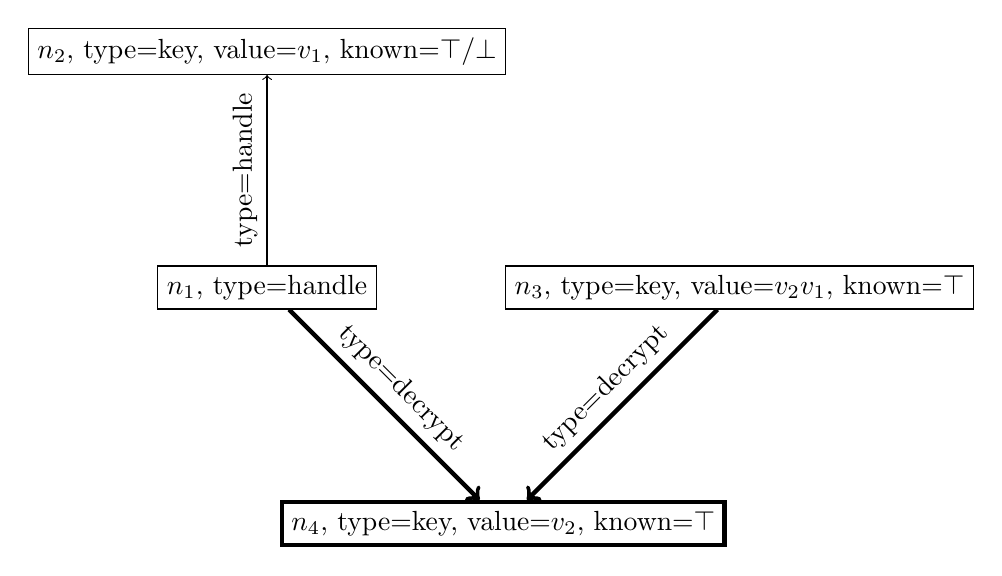
\begin{tikzpicture}
        \node (n2) at ( 0.0,  3.0) [draw, rectangle] {$n_2$, type=key, value=$v_1$, known=$\top/\bot$};
        \node (n3) at ( 6.0,  0.0) [draw, rectangle] {$n_3$, type=key, value=$\encryption{v_2}{v_1}$, known=$\top$};
        \node (n1) at ( 0.0,  0.0) [draw, rectangle] {$n_1$, type=handle};
        \node (n4) at ( 3.0, -3.0) [draw, rectangle, ultra thick] {$n_4$, type=key, value=$v_2$, known=$\top$};

        \draw[->] (n1) -- (n2) node[midway, sloped, above] {type=handle};
        \draw[->, ultra thick] (n1) -- (n4) node[midway, sloped, above] {type=decrypt};
        \draw[->, ultra thick] (n3) -- (n4) node[midway, sloped, above] {type=decrypt};
    \end{tikzpicture}
    \caption{Node $n_4$ does not exist. We add $n_4$ and edges $(n_1, n_4), (n_3, n_4)$ to it. We add command \texttt{decrypt(n1, n3)} to the alphabet.}
\end{figure}


\begin{figure}[h!]
    \centering
    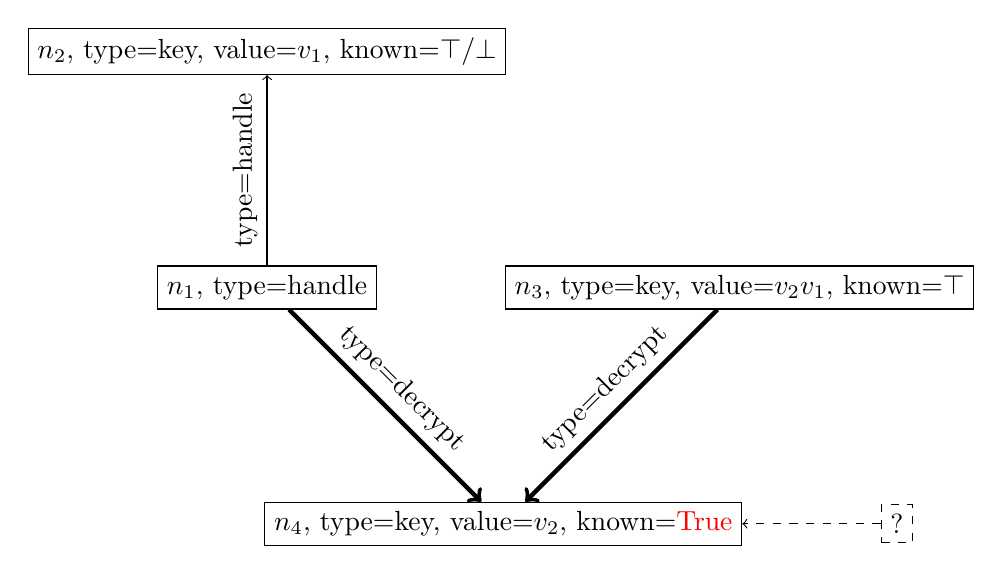
\begin{tikzpicture}
        \node (n2) at ( 0.0,   3.0) [draw, rectangle] {$n_2$, type=key, value=$v_1$, known=$\top/\bot$};
        \node (n3) at ( 6.0,   0.0) [draw, rectangle] {$n_3$, type=key, value=$\encryption{v_2}{v_1}$, known=$\top$};
        \node (n1) at ( 0.0,   0.0) [draw, rectangle] {$n_1$, type=handle};
        \node (n4) at ( 3.0,  -3.0) [draw, rectangle] {$n_4$, type=key, value=$v_2$, known=\textcolor{red}{True}};
        \node (p3) at ( 8.0,  -3.0) [draw, rectangle, dashed] {?};

        \draw[->] (n1) -- (n2) node[midway, sloped, above] {type=handle};
        \draw[->, ultra thick] (n1) -- (n4) node[midway, sloped, above] {type=decrypt};
        \draw[->, ultra thick] (n3) -- (n4) node[midway, sloped, above] {type=decrypt};
        \draw[->, dashed] (p3) -- (n4);
    \end{tikzpicture}
    \caption{Node $n_4$ already exists. If the pair of edges $(n_1, n_4), (n_3, n_4)$ does not already exist, we add it. We set $n_4$ as known. We add command \texttt{decrypt(n1, n3)} to the alphabet.}
\end{figure}

\newpage

\section*{Interesting cases}

\begin{figure}[h!]
    \centering
    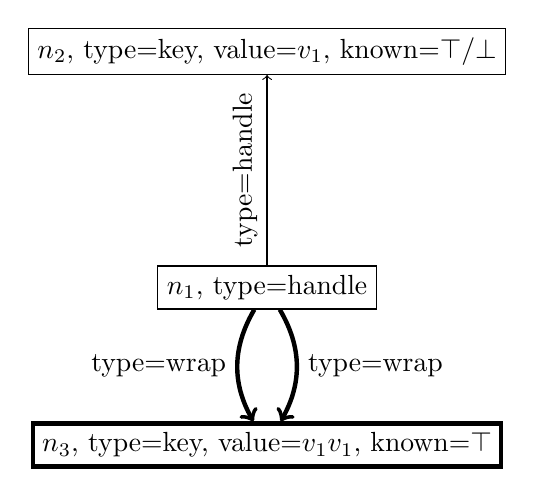
\begin{tikzpicture}
        \node (n2) at (0.0,  3.0) [draw, rectangle] {$n_2$, type=key, value=$v_1$, known=$\top/\bot$};
        \node (n1) at (0.0,  0.0) [draw, rectangle] {$n_1$, type=handle};
        \node (n3) at (0.0, -2.0) [draw, rectangle, ultra thick] {$n_3$, type=key, value=$\encryption{v_1}{v_1}$, known=$\top$};

        \draw[->] (n1) -- (n2) node[midway, sloped, above] {type=handle};
        \draw[->, bend left,  ultra thick] (n1) to node[midway, right] {type=wrap} (n3);
        \draw[->, bend right, ultra thick] (n1) to node[midway, left] {type=wrap} (n3);
    \end{tikzpicture}
    \caption{A handle node that wraps itself.}
\end{figure}

\begin{figure}[h!]
    \centering
    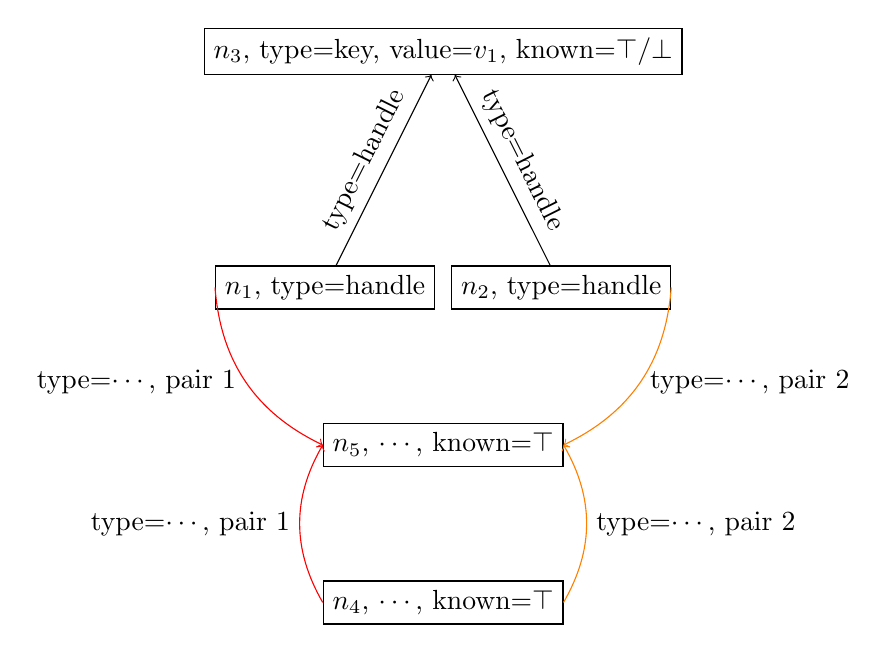
\begin{tikzpicture}
        \node (n3) at ( 0,  3.0) [draw, rectangle] {$n_3$, type=key, value=$v_1$, known=$\top/\bot$};
        \node (n1) at (-1.5,  0.0) [draw, rectangle] {$n_1$, type=handle};
        \node (n2) at ( 1.5,  0.0) [draw, rectangle] {$n_2$, type=handle};
        \node (n4) at ( 0.0, -4.0) [draw, rectangle] {$n_4$, $\cdots$, known=$\top$};
        \node (n5) at ( 0.0, -2.0) [draw, rectangle] {$n_5$, $\cdots$, known=$\top$};

        \draw[->] (n1) to node[midway, sloped, above]   {type=handle} (n3);
        \draw[->] (n2) to node[midway, sloped, above]  {type=handle} (n3);
        \draw[->, bend right, draw=red] (n1.west) to node[left] {type=$\cdots$, pair 1} (n5.west);
        \draw[->, bend left,  draw=red] (n4.west) to node[left] {type=$\cdots$, pair 1} (n5.west);
        \draw[->, bend left,  draw=orange]  (n2.east) to node[right] {type=$\cdots$, pair 2} (n5.east);
        \draw[->, bend right, draw=orange]  (n4.east) to node[right] {type=$\cdots$, pair 2} (n5.east);
    \end{tikzpicture}
    \caption{Two node handles to the same key appear in two distinct pair of edges that do the same production.}
\end{figure}

\newpage

\section*{Clulow's wrap and decrypt}

\begin{figure}[h!]
    \centering
    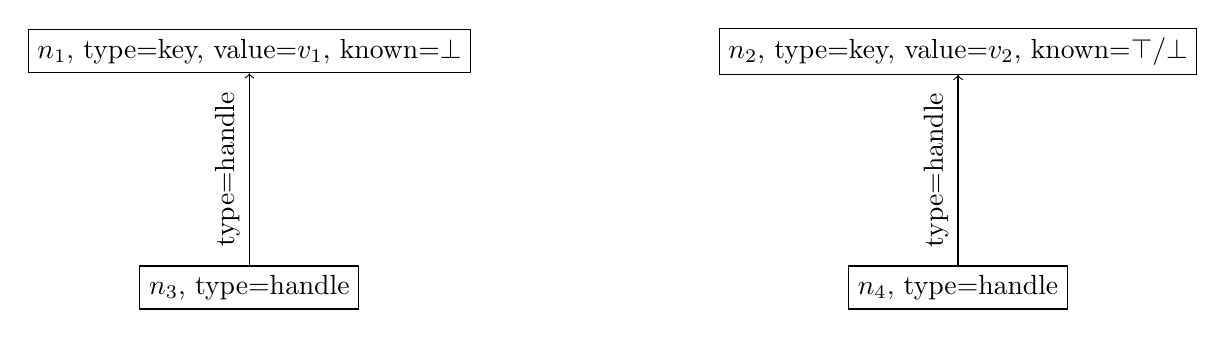
\begin{tikzpicture}
        \node (n1) at (0.0,  3.0) [draw, rectangle] {$n_1$, type=key, value=$v_1$, known=$\bot$};
        \node (n2) at (9.0,  3.0) [draw, rectangle] {$n_2$, type=key, value=$v_2$, known=$\top/\bot$};
        \node (n3) at (0.0,  0.0) [draw, rectangle] {$n_3$, type=handle};
        \node (n4) at (9.0,  0.0) [draw, rectangle] {$n_4$, type=handle};

        \draw[->] (n3) -- (n1) node[midway, sloped, above] {type=handle};
        \draw[->] (n4) -- (n2) node[midway, sloped, above] {type=handle};
    \end{tikzpicture}
    \caption{Initial state.}
\end{figure}

\begin{figure}[h!]
    \centering
    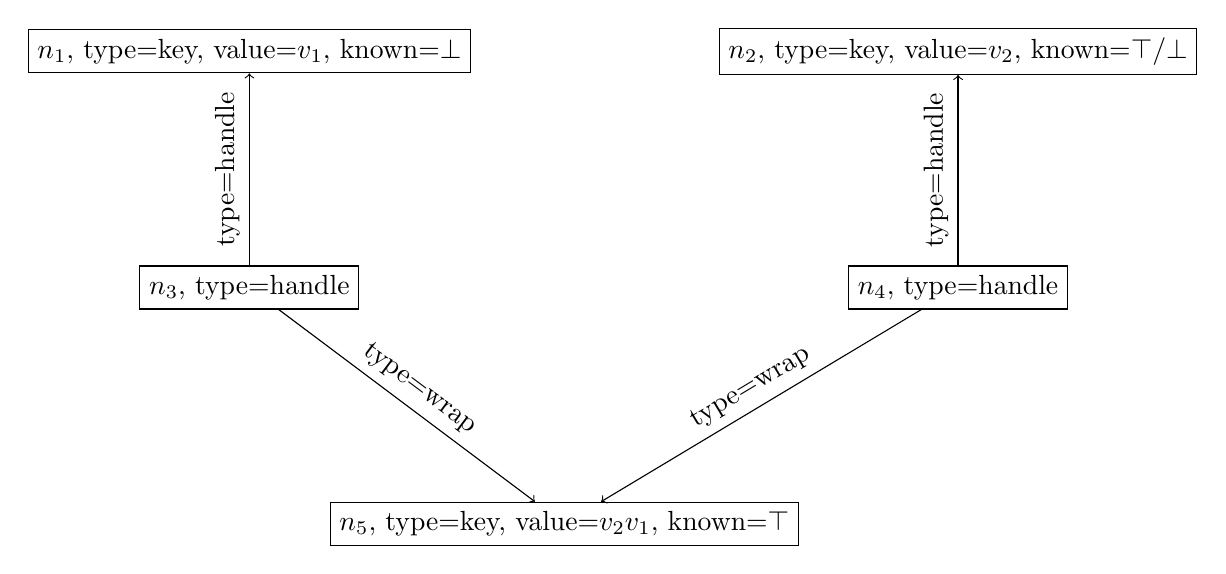
\begin{tikzpicture}
        \node (n1) at (0.0,  3.0) [draw, rectangle] {$n_1$, type=key, value=$v_1$, known=$\bot$};
        \node (n2) at (9.0,  3.0) [draw, rectangle] {$n_2$, type=key, value=$v_2$, known=$\top/\bot$};
        \node (n3) at (0.0,  0.0) [draw, rectangle] {$n_3$, type=handle};
        \node (n4) at (9.0,  0.0) [draw, rectangle] {$n_4$, type=handle};
        \node (n5) at (4.0, -3.0) [draw, rectangle] {$n_5$, type=key, value=$\encryption{v_2}{v_1}$, known=$\top$};

        \draw[->] (n3) -- (n1) node[midway, sloped, above] {type=handle};
        \draw[->] (n4) -- (n2) node[midway, sloped, above] {type=handle};
        \draw[->] (n3) -- (n5) node[midway, sloped, above] {type=wrap};
        \draw[->] (n4) -- (n5) node[midway, sloped, above] {type=wrap};
    \end{tikzpicture}
    \caption{Wrap. Add command \texttt{wrap(n3, n4)} to the alphabet.}
\end{figure}

\begin{figure}[h!]
    \centering
    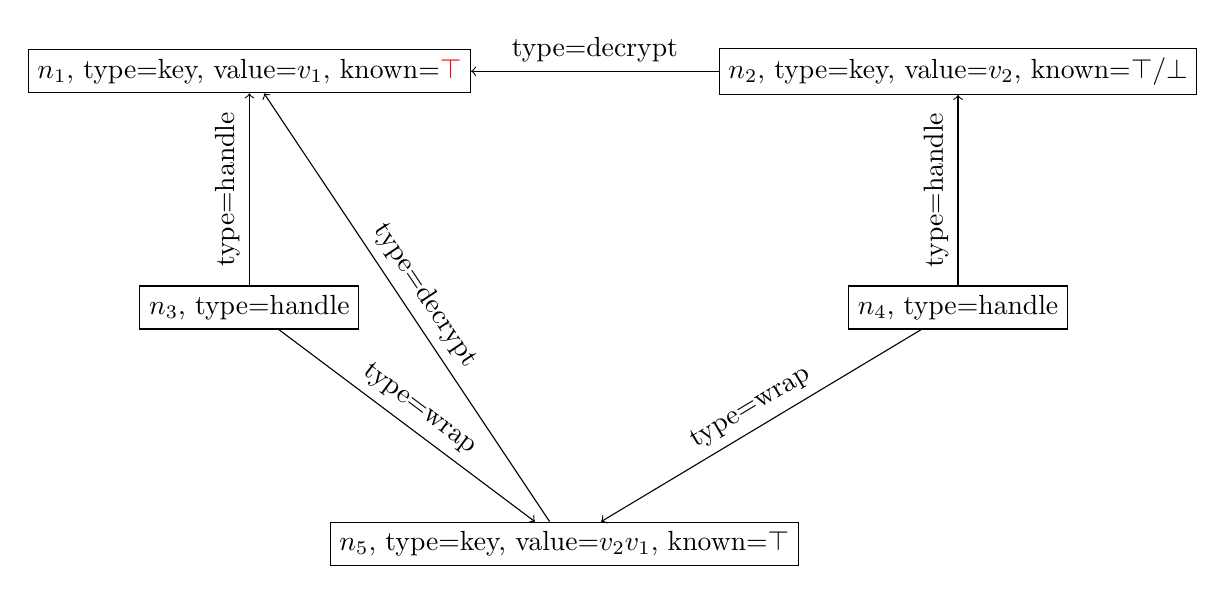
\begin{tikzpicture}
        \node (n1) at (0.0,  3.0) [draw, rectangle] {$n_1$, type=key, value=$v_1$, known=\textcolor{red}{$\top$}};
        \node (n2) at (9.0,  3.0) [draw, rectangle] {$n_2$, type=key, value=$v_2$, known=$\top/\bot$};
        \node (n3) at (0.0,  0.0) [draw, rectangle] {$n_3$, type=handle};
        \node (n4) at (9.0,  0.0) [draw, rectangle] {$n_4$, type=handle};
        \node (n5) at (4.0, -3.0) [draw, rectangle] {$n_5$, type=key, value=$\encryption{v_2}{v_1}$, known=$\top$};

        \draw[->] (n3) -- (n1) node[midway, sloped, above] {type=handle};
        \draw[->] (n4) -- (n2) node[midway, sloped, above] {type=handle};
        \draw[->] (n3) -- (n5) node[midway, sloped, above] {type=wrap};
        \draw[->] (n4) -- (n5) node[midway, sloped, above] {type=wrap};
        \draw[->] (n5) -- (n1) node[midway, sloped, above] {type=decrypt};
        \draw[->] (n2) -- (n1) node[midway, sloped, above] {type=decrypt};
    \end{tikzpicture}
    \caption{Decrypt. Add command \texttt{decrypt(n2, n5)} to the alphabet.}
\end{figure}

\newpage

\section{Algorithms}

\begin{algorithm}
    \caption{Wrap}
    \begin{algorithmic}
        \Require $G_0$
        \Ensure $G_1$
        \State $G_1 \gets \copygraph{G_0}$

        \ForAll{$\node{n_1}, \node{n_2} \in \graph{G_0} \mid \handle{\node{n_1}} = \top, \key{\node{n_2}} = \top, v_1 = \valueof{n_2}, \handle{(\node{n_1}, \node{n_2})} = \top$}

        \ForAll{$\node{n_3}, \node{n_4} \in \graph{G_0} \mid \handle{\node{n_3}} = \top, \key{\node{n_4}} = \top, v_2 = \valueof{n_4}, \handle{(\node{n_3}, \node{n_4})} = \top$}

        \If{$n_5 \notin G_1 \mid \key{n_5} = \top, \valueof{\node{n_5}} = \encryption{v_2}{v_1}$}
        \State $G_1 \gets G_1 \cup \{ \node{n_5} \mid \key{\node{n_5}} = \top, \valueof{\node{n_5}} = \encryption{v_2}{v_1}, \known{\node{n_5}} = \top \}$
        \State $G_1 \gets G_1 \cup \{ \edge{n_1}{n_5} \mid \wrap{\edge{n_1}{n_5}} = \top \}$
        \State $G_1 \gets G_1 \cup \{ \edge{n_3}{n_5} \mid \wrap{\edge{n_3}{n_5}} = \top \}$
        \Else
        \If{$\edge{n_1}{n_5}, \edge{n_3}{n_5} \notin \graph{G_1} \mid \wrap{\edge{n_1}{n_5}} = \top, \wrap{\edge{n_3}{n_5}} = \top$}
        \State $G_1 \gets G_1 \cup \{ \edge{n_1}{n_5} \mid \wrap{\edge{n_1}{n_5}} = \top \}$
        \State $G_1 \gets G_1 \cup \{ \edge{n_3}{n_5} \mid \wrap{\edge{n_3}{n_5}} = \top \}$
        \EndIf
        \If{$\known{\node{n_5}} = \bot$}
        \State $\known{\node{n_5}} = \top$
        \EndIf
        \EndIf
        \EndFor
        \EndFor
    \end{algorithmic}
\end{algorithm}

\begin{algorithm}
    \caption{Encrypt}
    \begin{algorithmic}
        \Require $G_0$
        \Ensure $G_1$
        \State $G_1 \gets \copygraph{G_0}$

        \ForAll{$\node{n_1}, \node{n_2} \in \graph{G_0} \mid \handle{\node{n_1}} = \top, \key{\node{n_2}} = \top, v_1 = \valueof{n_2}, \handle{(\node{n_1}, \node{n_2})} = \top$}

        \ForAll{$\node{n_3} \in \graph{G_0} \mid \key{\node{n_3}} = \top, v_2 = \valueof{n_3}, \known{\node{m_3}} = \top$}

        \If{$n_4 \notin G_1 \mid \key{n_4} = \top, \valueof{\node{n_4}} = \encryption{v_2}{v_1}$}
        \State $G_1 \gets G_1 \cup \{ \node{n_4} \mid \key{\node{n_4}} = \top, \valueof{\node{n_4}} = \encryption{v_2}{v_1}, \known{\node{n_4}} = \top \}$
        \State $G_1 \gets G_1 \cup \{ \edge{n_1}{n_4} \mid \encrypt{\edge{n_1}{n_4}} = \top \}$
        \State $G_1 \gets G_1 \cup \{ \edge{n_3}{n_4} \mid \encrypt{\edge{n_3}{n_4}} = \top \}$
        \Else
        \If{$\edge{n_1}{n_4}, \edge{n_3}{n_4} \notin \graph{G_1} \mid \encrypt{\edge{n_1}{n_4}} = \top, \encrypt{\edge{n_3}{n_4}} = \top \}$}
        \State $G_1 \gets G_1 \cup \{ \edge{n_1}{n_4} \mid \encrypt{\edge{n_1}{n_4}} = \top \}$
        \State $G_1 \gets G_1 \cup \{ \edge{n_3}{n_4} \mid \encrypt{\edge{n_3}{n_4}} = \top \}$
        \EndIf
        \If{$\known{\node{n_4}} = \bot$}
        \State $\known{\node{n_4}} = \top$
        \EndIf
        \EndIf
        \EndFor
        \EndFor
    \end{algorithmic}
\end{algorithm}

\begin{algorithm}
    \caption{Unwrap}
    \begin{algorithmic}
        \Require $G_0$
        \Ensure $G_1$
        \State $G_1 \gets \copygraph{G_0}$

        \ForAll{$\node{n_1}, \node{n_2} \in \graph{G_0} \mid \handle{\node{n_1}} = \top, \key{\node{n_2}} = \top, v_1 = \valueof{n_2}, \handle{(\node{n_1}, \node{n_2})} = \top$}

        \ForAll{$\node{n_3} \in \graph{G_0} \mid \key{\node{n_3}} = \top, \encryption{v_2}{v_1} = \valueof{n_3}, \known{\node{n_3}} = \top$}

        \If{$n_4 \notin G_1 \mid \key{n_4} = \top, \valueof{\node{n_4}} = v_2$}
        \State $G_1 \gets G_1 \cup \{ \node{n_4} \mid \key{\node{n_4}} = \top, \valueof{\node{n_4}} = v_2, \known{\node{n_4}} = \top \}$
        \State $G_1 \gets G_1 \cup \{ \node{n_5} \mid \handle{\node{n_5}} = \top \}$
        \State $G_1 \gets G_1 \cup \{ \edge{n_1}{n_5} \mid \unwrap{\edge{n_1}{n_5}} = \top \}$
        \State $G_1 \gets G_1 \cup \{ \edge{n_3}{n_5} \mid \unwrap{\edge{n_3}{n_5}} = \top \}$
        \State $G_1 \gets G_1 \cup \{ \edge{n_5}{n_4} \mid \handle{\edge{n_5}{n_4}} = \top \}$
        \Else
        \If{$|n \mid (n, n_5) \in \graph{G}, \handle{n, n_5}| < 2$}
        \State $G_1 \gets G_1 \cup \{ \node{n_5} \mid \handle{\node{n_5}} = \top \}$
        \State $G_1 \gets G_1 \cup \{ \edge{n_1}{n_5} \mid \unwrap{\edge{n_1}{n_5}} = \top \}$
        \State $G_1 \gets G_1 \cup \{ \edge{n_3}{n_5} \mid \unwrap{\edge{n_3}{n_5}} = \top \}$
        \State $G_1 \gets G_1 \cup \{ \edge{n_5}{n_4} \mid \handle{\edge{n_5}{n_4}} = \top \}$
        \EndIf
        \EndIf
        \EndFor
        \EndFor
    \end{algorithmic}
\end{algorithm}

\begin{algorithm}
    \caption{Decrypt}
    \begin{algorithmic}
        \Require $G_0$
        \Ensure $G_1$
        \State $G_1 \gets \copygraph{G_0}$

        \ForAll{$\node{n_1}, \node{n_2} \in \graph{G_0} \mid \handle{\node{n_1}} = \top, \key{\node{n_2}} = \top, v_1 = \valueof{n_2}, \handle{(\node{n_1}, \node{n_2})} = \top$}

        \ForAll{$\node{n_3} \in \graph{G_0} \mid \key{\node{n_3}} = \top, \encryption{v_2}{v_1} = \valueof{n_3}, \known{\node{m_3}} = \top$}

        \If{$n_4 \notin G_1 \mid \key{n_4} = \top, \valueof{\node{n_4}} = v_2$}
        \State $G_1 \gets G_1 \cup \{ \node{n_4} \mid \key{\node{n_4}} = \top, \valueof{\node{n_4}} = v_2, \known{\node{n_4}} = \top \}$
        \State $G_1 \gets G_1 \cup \{ \edge{n_1}{n_4} \mid \decrypt{\edge{n_1}{n_4}} = \top \}$
        \State $G_1 \gets G_1 \cup \{ \edge{n_3}{n_4} \mid \decrypt{\edge{n_3}{n_4}} = \top \}$
        \Else
        \If{$\edge{n_1}{n_4}, \edge{n_3}{n_4} \notin \graph{G_1} \mid \decrypt{\edge{n_1}{n_4}} = \top, \decrypt{\edge{n_3}{n_4}} = \top $}
        \State $G_1 \gets G_1 \cup \{ \edge{n_1}{n_4} \mid \decrypt{\edge{n_1}{n_4}} = \top \}$
        \State $G_1 \gets G_1 \cup \{ \edge{n_3}{n_4} \mid \decrypt{\edge{n_3}{n_4}} = \top \}$
        \EndIf
        \If{$\known{\node{n_4}} = \bot$}
        \State $\known{\node{n_4}} = \top$
        \EndIf
        \EndIf
        \EndFor
        \EndFor
    \end{algorithmic}
\end{algorithm}

\end{document}
